\documentclass[11pt]{article}
\usepackage[T1]{fontenc}
\usepackage[margin=1.25in]{geometry}
\usepackage[expansion=false]{microtype}
\usepackage{amsmath,amssymb}
\usepackage{booktabs,tabularx,array}
\usepackage{enumitem}
\usepackage{tikz}
\usetikzlibrary{arrows.meta}
\usepackage{hyperref}
\emergencystretch=3em
\setlength{\parskip}{0.55em}
\setlength{\parindent}{0pt}

\newcommand{\IN}{\textsf{IN}}
\newcommand{\UND}{\textsf{UND}}
\newcommand{\OUT}{\textsf{OUT}}

\title{Disagreement Has Four Causes}
\author{Flyxion\\\small Independent Researcher}
\date{30 September 2026}

\begin{document}
\maketitle

\begin{abstract}
\noindent
Two people who say ``that is wrong'' and ``that is right'' about the same claim are often in one of four quite different situations. Nothing has been argued at the place in question. Two arguments oppose each other on equal footing. An argument stands or falls on an attack on its method that nobody has answered. Or the two sides are speaking about different parts of the territory and never meet. Each situation leaves a distinct signature in a record that keeps what has been argued apart from what stands, and each calls for a different kind of move. This guide states the four signatures, gives a flowchart for telling them apart, and gives one short invented example of each, including a methodological attack recorded as a one-sided state. It is written for editors, moderators and working scientists. The signatures are a result of the monograph \emph{Adversaria: A Specification for a Public Claim Graph}; the advice about moves is practice and not a theorem. Naming the situation does not settle the dispute, and the four situations are not claimed to cover every kind of disagreement.
\end{abstract}

\section{Why diagnose before arguing}

Most stalled disputes stall because the participants are answering a question the other side did not ask. One party keeps adding sources, the other keeps saying the sources are beside the point. One party asks for a ruling, the other says the question is ill-posed. A moderator who sees only the heat of the exchange can do little except ask for calm or pick a side.

A record that separates two things can do better. The first is what has been put on the table: which arguments exist, for which claims, over which region. The second is what stands: which of those arguments survive every objection that has been filed against them, under a stated way of preferring one argument to another. When those two layers are kept apart, the pattern of the dispute shows in the pair of them, and the pattern tells the participants what kind of move could change anything.

This guide is about four patterns. They are not a theory of why people disagree in general. They are four situations that a claim graph can distinguish mechanically, and that cover the cases an editor most often meets. A dispute that matches none of them is reported as such, and Section~\ref{sec:none} says how.

\section{The vocabulary in one page}\label{sec:vocab}

The monograph is the source of every definition here; this section restates only what the guide uses.

A \emph{unit} is one combination of values along the dimensions a claim is about, such as a population, a setting, a period or a measurement regime. A \emph{scope} is a set of units. A \emph{claim} asserts a kernel, a precisely stated proposition with its own negation, over a scope. The negation of a claim's kernel is written with a bar here: the claim ``the effect holds'' and the claim ``the effect fails'' have opposite kernels (Chapter 4).

An \emph{argument} offers a claim on the strength of evidence and a warrant that connects the two. An objection is not a comment. It is an argument whose conclusion denies a part of another argument, and there are three kinds (Chapter 7). A \emph{rebuttal} concludes the opposite of the target's conclusion. An \emph{undermining} attack concludes that a piece of evidence is not accurate or not applicable at the unit. An \emph{undercutting} attack concludes that the warrant, the step from evidence to claim, does not hold at the unit. The second and third are what this guide calls \emph{methodological} attacks: they do not say the conclusion is false, they say the route to it is broken. Each attack has an active region, the units where the attacker, the target and the target's component all exist, and an attack on no shared unit does not count.

At each unit, each argument present carries one of three \emph{labels}, computed from the attacks by the grounded rule of Chapter 7. An argument is \IN{} if every attacker of it is \OUT{}. It is \OUT{} if some attacker of it is \IN{}. It is \UND{} otherwise, which means that it is neither established nor refuted under the rules. A label is a statement of standing under a policy and a record. It is not truth.

The \emph{evidential state} at a unit is a separate, purely informational reading of who has argued what (Chapter 12). It takes one of four values.
\begin{center}
\begin{tabular}{@{}cl@{}}
\toprule
value & meaning\\
\midrule
$\mathsf T$ & an argument for the claim is present at the unit, and none for the opposite kernel\\
$\mathsf F$ & an argument for the opposite kernel is present, and none for the claim\\
$\mathsf B$ & arguments on both sides are present\\
$\mathsf N$ & neither\\
\bottomrule
\end{tabular}
\end{center}
These four symbols are borrowed from a classical four-valued logic, and they must be read as a ledger of what has been told. $\mathsf T$ does not mean true and $\mathsf F$ does not mean false. $\mathsf B$ does not mean the store is broken, and $\mathsf N$ does not mean the claim is unknown in any deep sense. They say whether argument exists. The labels say how that argument fares.

Two facts from the model are used throughout. A claim's conclusion is never given a standing it has not earned by the mere presence of a conflict (Chapter 7, the corollary on non-explosion). And the record keeps stance separate from argument: any number of people recording agreement or rejection changes no label (Chapter 12).

\section{The four signatures}\label{sec:signatures}

Chapter 12 proves that four situations occur and that no two of them produce the same pair of evidential state and labels. The pair is the signature.

\begin{center}
\small
\begin{tabularx}{\textwidth}{@{}>{\raggedright\arraybackslash}p{0.2\textwidth} l X@{}}
\toprule
situation & state & labels of the arguments for the claim\\
\midrule
lack of evidence & $\mathsf N$ & no argument present\\
balanced conflict & $\mathsf B$ & arguments for and against both \UND{}, each held up only by the other's rebuttal\\
unresolved methodological attack & $\mathsf T$ or $\mathsf F$ & the argument is \UND{} because an undermining or undercutting attacker is \UND{}\\
scope mismatch & $\mathsf T$ at some units, $\mathsf F$ at others, never $\mathsf B$ & arguments on both sides exist, but their scopes are disjoint\\
\bottomrule
\end{tabularx}
\end{center}

The proof in the monograph is constructive: for each row it exhibits a small ledger that produces the signature. For a balanced conflict the ledger is two arguments with opposite conclusions and overlapping scope and nothing else (Chapter 7 shows that they are then both \UND{}, and that an acyclic dispute is never left open). For an unresolved methodological attack it is an argument, an undercutter of its warrant, and a counter-argument that the warrant is sound, which rebuts the undercutter as the undercutter rebuts it. For scope mismatch it is two arguments with opposite kernels on disjoint scopes. The examples in Section~\ref{sec:cases} are instances of these constructions, and their labels were checked by computation (Section~\ref{sec:check}).

Three cautions belong here. First, the table is a statement about what occurs and what can be told apart. It is not a statement that these are the only ways a unit can look. Second, the signatures are read at a unit, and scope mismatch is read across units, since it is a fact about where two bodies of argument lie. Third, the proposition says the four are distinguishable by signature. Whether a real dispute has the signature depends on what has actually been inscribed, and that can be wrong or incomplete.

\section{A flowchart for telling them apart}\label{sec:flow}

The diagnosis starts from a claim and a unit where the disagreement is located. If the dispute is over a whole region, run the chart for a representative unit of each piece of the region that the two parties are quoting.

\begin{figure}[ht]
\centering
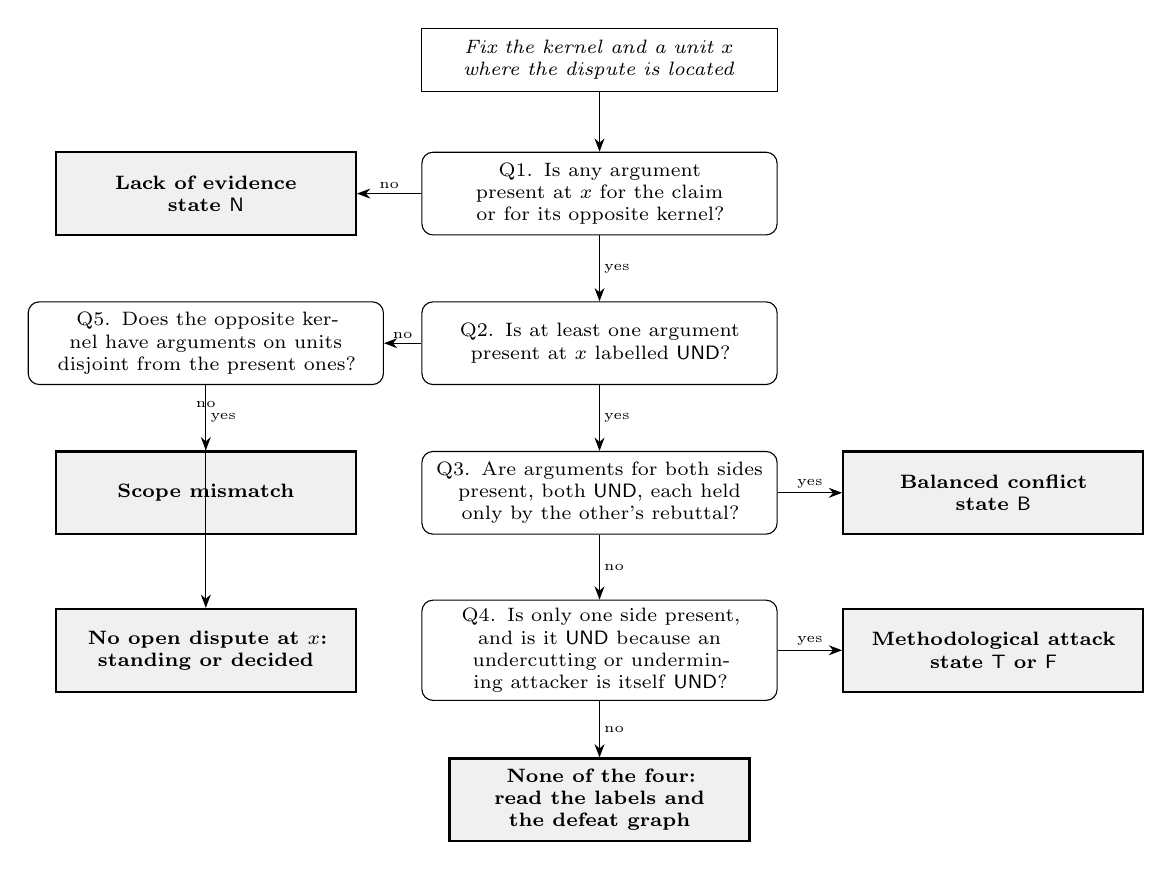
\begin{tikzpicture}[
  x=1cm,y=1cm,
  >=Stealth,
  dec/.style={draw,rounded corners=4pt,align=center,text width=4.3cm,minimum height=1.05cm,font=\scriptsize,inner sep=3pt},
  term/.style={draw,thick,align=center,text width=3.6cm,minimum height=1.05cm,font=\scriptsize\bfseries,inner sep=3pt,fill=black!6},
  start/.style={draw,align=center,text width=4.3cm,minimum height=0.8cm,font=\scriptsize\itshape,inner sep=3pt},
  lab/.style={font=\tiny,inner sep=1.5pt}
]
\node[start] (s) at (0,0) {Fix the kernel and a unit $x$ where the dispute is located};
\node[dec] (q1) at (0,-1.7) {Q1. Is any argument present at $x$ for the claim or for its opposite kernel?};
\node[dec] (q2) at (0,-3.6) {Q2. Is at least one argument present at $x$ labelled \UND{}?};
\node[dec] (q3) at (0,-5.5) {Q3. Are arguments for both sides present, both \UND{}, each held only by the other's rebuttal?};
\node[dec] (q5) at (0,-7.5) {Q4. Is only one side present, and is it \UND{} because an undercutting or undermining attacker is itself \UND{}?};
\node[term] (lack) at (-5.0,-1.7) {Lack of evidence\\ state $\mathsf N$};
\node[dec] (q6) at (-5.0,-3.6) {Q5. Does the opposite kernel have arguments on units disjoint from the present ones?};
\node[term] (scope) at (-5.0,-5.5) {Scope mismatch};
\node[term] (settled) at (-5.0,-7.5) {No open dispute at $x$:\\ standing or decided};
\node[term] (bal) at (5.0,-5.5) {Balanced conflict\\ state $\mathsf B$};
\node[term] (meth) at (5.0,-7.5) {Methodological attack\\ state $\mathsf T$ or $\mathsf F$};
\node[term] (other) at (0,-9.4) {None of the four: read the labels and the defeat graph};
\draw[->] (s) -- (q1);
\draw[->] (q1) -- node[lab,right]{yes} (q2);
\draw[->] (q1) -- node[lab,above]{no} (lack);
\draw[->] (q2) -- node[lab,right]{yes} (q3);
\draw[->] (q2) -- node[lab,above]{no} (q6);
\draw[->] (q6) -- node[lab,right]{yes} (scope);
\draw[->] (q6.south) -- ++(0,-0.35) -| node[lab,pos=0.2,above]{no} (settled.north);
\draw[->] (q3) -- node[lab,above]{yes} (bal);
\draw[->] (q3) -- node[lab,right]{no} (q5);
\draw[->] (q5) -- node[lab,above]{yes} (meth);
\draw[->] (q5) -- node[lab,right]{no} (other);
\end{tikzpicture}
\caption{Flowchart for the four situations at a unit. The terminal boxes are shaded. Questions are asked from the top, and the shaded boxes end the diagnosis.}\label{fig:flow}
\end{figure}

Reading notes for the chart.

\begin{itemize}[nosep]
\item Q1 and Q2 are questions about the record at the unit. They are answered from the evidential state and from the labels that the dossier already displays.
\item Q3 is the test for a balanced conflict. The phrase ``held only by the other's rebuttal'' matters: if either side has some further attacker, the case belongs in the last box, not in this one.
\item Q4 separates a methodological attack from everything else that can leave a one-sided argument unresolved. The requirement that the attacker itself be \UND{} is what makes the situation unresolved and not merely contested: an undercutter that has been answered by a standing reply is \OUT{}, and the argument it attacked is restored.
\item Q5 is asked only when nothing is open at $x$. It is how the chart finds a scope mismatch: each side is settled where it speaks, and the opposition is a matter of where they speak.
\item When the box ``none of the four'' is reached, the dispute needs the defeat graph read directly. Section~\ref{sec:none} gives two common cases.
\end{itemize}

\section{Four cases, one invented claim}\label{sec:cases}

One schematic claim serves for all four cases. Everything in it is invented and no result is reported. Let the kernel $K$ say that spraying a fermented compost tea on bean plots raises the harvested yield by at least five percent, with yield measured as the dry mass of shelled beans per plot. The units have two dimensions: soil (clay $C$, sand $S$) and season (wet $W$, dry $D$). The four units are $CW$, $CD$, $SW$, $SD$. Trials are invented and lettered.

\subsection{Lack of evidence}

\emph{Situation.} Two editors disagree about whether the tea works on sandy soil in a dry season. One says it obviously does, since it works on clay. The other says there is no reason to think so. Nothing has been inscribed at $SD$. The only argument in the dossier is one from trial A, concluding $K$ over $CW$.

\emph{Signature.} At $SD$ the evidential state is $\mathsf N$ and no argument is present. The argument from trial A is \IN{} at $CW$ and is not present anywhere else.

\emph{What kind of move settles it.} Only a move that adds argument at $SD$ changes the signature: a trial on sandy plots in a dry season, a warrant for carrying a result across soils with backing, or an observational record. The monograph makes the reason exact in two places. A scope is part of what a claim says. Narrowing a claim never breaks it, and a claim over a union of scopes holds exactly when it holds over each part (Chapter 4), so widening a claim adds a burden that the original argument did not carry. A well-formed argument cannot conclude a scope beyond what its premises cover (condition W1, Chapter 6), so an argument for $K$ over $CW$ supports nothing over $SD$. Carrying a result across soils needs a further warrant, and that warrant is open to attack (Chapter 8 proves the corresponding fact for senses of a term).

\emph{What does not settle it.} Repeating the editor's confidence, recording more agreement, or asking the other editor to disprove the claim. The second editor owes no argument, because no argument has been offered at $SD$. Recorded agreement has no defeat power and no evidential weight in the model (Chapter 12).

\subsection{Balanced conflict}

\emph{Situation.} Trial B, on clay plots in both seasons, found a yield gain of eight percent, and its authors inscribe an argument for $K$ over $CW$ and $CD$. Trial C, on clay in the wet season only, found no gain, and its authors inscribe an argument for $\bar K$ over $CW$ from a bounded-effect design. Nobody has attacked the evidence or the method of either trial. Neither argument is preferred to the other by the policy in force.

\emph{Signature.} At $CD$ the evidential state is $\mathsf T$ and the argument from trial B is \IN{}. At $CW$ the state is $\mathsf B$ and the two arguments rebut each other, neither has any other attacker, and both are \UND{}. This is the exact content of the statement in Chapter 7 that a symmetric defeat stays open: the grounded rule never picks a winner by fiat. The labels were computed and agree.

\emph{What kind of move settles it.} Three kinds of move change the labels, and they differ in what they say.
\begin{enumerate}[nosep]
\item A \emph{reply}: a new argument that defeats one of the two, typically by attacking its evidence or method. If it stands, the attacked argument goes \OUT{} and the other is reinstated (Chapter 7).
\item A \emph{preference}: a policy, itself a ledger object, that ranks one argument below the other on the region. Preferences are regional and are open to objection like anything else. A policy that prefers preregistered trials is a choice about what to prize and it does not say which result is right. The same ledger under two policies can carry different labels with no inconsistency (Chapter 7, the theorem on policy-relative defeat).
\item A \emph{constraint}: if the clash covers only part of a larger claim, the parties can agree to state what survives. Here the claim is asserted over $CW$ and $CD$ and trial C concerns only $CW$, so under the default policy the claim stands at $CD$ and is open at $CW$ (Chapter 7, scoped disagreement). The survivor is the claim restricted to $CD$ (Chapter 11). This does not close the question at $CW$. It removes $CD$ from the quarrel and leaves the quarrel where it lives.
\end{enumerate}
The scope remaining after several such limits depends on the set of limits and not on the order in which they were filed (Chapter 11). That is a fact about scopes; the labels are read from the ledger.

\emph{What does not settle it.} Inscribing trial B's result ten times, or having ten reviewers record the same stance. Replication is counted by independent families of evidence and never by records (Chapter 5), and stance changes no label.

\subsection{Unresolved methodological attack}

\emph{Situation.} Trial D, on clay in a wet season, measured yield by weighing whole plots, and its authors inscribe an argument for $K$ over $CW$ using the warrant that plot mass tracks shelled-bean mass. A reader files an undercutter: in a wet season the plots carried wet pods, so the warrant fails at $CW$. The authors file a counter-argument that the warrant is sound, because pods were dried to a constant mass before weighing. The undercutter concludes that the warrant does not hold, and the counter-argument concludes that it does, so each rebuts the other with the same region.

\emph{Signature.} At $CW$ the evidential state is $\mathsf T$, because the only argument on the question of $K$ is the one for it. The undercutter and the counter-argument conclude things about the warrant, not about $K$, so neither counts as an argument against the claim. All three arguments are \UND{}: the argument from trial D is \UND{} because its undercutter is \UND{}. This matches the third row of the table, and the computation confirms it.

The state is $\mathsf T$ here because the attacked argument is on the claim's side. If the attacked argument were the one from trial C for $\bar K$, the same three-argument structure would give state $\mathsf F$, and the labels would be identical. The letter reports which side has argued. It does not say which side is in trouble, and it should not be read as a verdict.

\emph{What kind of move settles it.} A move that breaks the tie between undercutter and counter-argument. Typical ones are a reply that undermines the evidence of the undercutter (for instance, showing that the observation of wet pods was from a different field); a record of the drying protocol that makes the undercutter's premise inapplicable; or a policy preference on this region between the two. With the first of these the undercutter goes \OUT{}, the counter-argument is unattacked and \IN{}, and the argument from trial D is \IN{}; the computation confirms this for the invented case. The move has to address the method. Adding more trials of the same design does not answer an undercutter of the warrant that connects those trials to yield. A new trial that measures shelled beans directly is, however, a different argument with a different warrant, and it supports $K$ without relying on the contested one.

\emph{What does not settle it.} Arguing about whether $K$ is true. The unresolved thing is whether a route to $K$ is sound, and the dispute about the conclusion is downstream of it. The monograph also ties the attack to its target: an attack on the warrant bites every argument that uses that warrant, on the region each of them reaches (Chapter 7), so the same undercutter will later be raised against any other plot-mass trial. That is often the most useful thing a moderator can point out.

\subsection{Scope mismatch}

\emph{Situation.} Trial A and trial F are both sound and unchallenged. Trial A, on clay in both seasons, supports $K$ over $CW$ and $CD$. Trial F, on sandy plots in both seasons, found no gain, and supports $\bar K$ over $SW$ and $SD$. A reader who sees both headlines says the literature is split. One who sees only trial A says the tea works. One who sees only trial F says it does not.

\emph{Signature.} The evidential state is $\mathsf T$ on the clay units and $\mathsf F$ on the sandy units and $\mathsf B$ nowhere. Each argument is \IN{} on its own scope. The monograph states this shape directly: two arguments with opposite kernels and disjoint scopes do not attack each other, since an attack needs a nonempty active region, and the claims are jointly satisfiable exactly when their scopes do not overlap (Chapter 4, conflict localization).

\emph{What kind of move settles it.} Often none is needed at the level of labels, since nothing is in conflict. The useful move is to state the two claims with their scopes so that nobody quotes one as though it covered the other, and then to ask whether the boundary follows a real difference, here soil, that a mechanism or further trials could explain. If it does, that is a finding. A claim can also be stated as pooled over the two regions, and then it is supported where its sub-arguments are and unaddressed elsewhere.

A related case deserves its own paragraph, because it often looks like a balanced conflict. Suppose the dispute turns on a word. One party measured fresh pod mass and another measured dry bean mass, and each calls their measure ``yield.'' Both parties quote the same sentence and seem to overlap. The monograph's remedy is a \emph{pooling declaration}: a record stating that the umbrella term is overloaded and naming the kernels for each sense, with the meaning of the umbrella claim fixed as the sense-by-sense reading of its parts. The declaration changes no existing record, and it is itself open to argument. By the decomposition theorem, a claim about the umbrella term over a scope is exactly the conjunction of claims about each sense over that scope's slice of the sense dimension, and by the companion result no finding about some senses supports the umbrella claim over a slice belonging to another (Chapter 8). Once each party restates the finding as the claim their evidence supports, for the sense they measured, the two claims have different kernels. Attack is defined from equal and opposite kernels (Chapter 7), so they do not attack each other. What looked like a balanced conflict on the umbrella term becomes a difference of scope along the sense dimension. The declaration does not decide whether the umbrella claim holds, and the original opposing arguments remain in the ledger.

\emph{What does not settle it.} Taking a vote on whether the tea works. A vote about the pooled statement decides nothing about either region and has no standing in the labels.

\section{Checking the examples}\label{sec:check}

The labels stated in the four cases were checked by a short program that builds the small regional frameworks described above, derives the attacks from the conclusion kernels as in Chapter 7, and computes the grounded labeling at each of the four units. The program reproduced the signature stated for each case. It also reproduced three variations used in the text: the methodological structure with the attacked argument on the opposing side, which gives state $\mathsf F$ with the same labels; the methodological case with a standing reply that undermines the undercutter's evidence, which returns the attacked argument to \IN{}; and the balanced case with a policy preference, which resolves it on the preferred region. This is a check of the examples against the stated definitions. It is not an empirical result, and the trials and numbers are invented.

\section{When none of the four fits}\label{sec:none}

The proposition does not say that every disagreement is one of these. Two patterns that editors meet often fall outside.

\emph{A dispute that is already decided.} Suppose a balanced conflict at $CW$ is followed by a reply that undermines the evidence of the side against $K$. The state is still $\mathsf B$, since arguments for both sides are present, but the labels are now \IN{} for the pro side and \OUT{} for the con side, and the reply is \IN{}. The record contains a disagreement, and the disagreement has been resolved under the policy. The flowchart sends this case to the box ``no open dispute.'' That is not a statement that the losing side is wrong. The labels record standing under a policy, and a party who rejects the policy is raising the next case.

\emph{A dispute about the policy.} Two communities can hold every record in common and differ only in how they prefer one argument to another. Their dossiers then differ, and the difference is traceable to the policy and to nothing else (Chapter 9, the theorem on traceable divergence; Chapter 7 gives a two-policy example on one ledger). Such a disagreement can look like a balanced conflict, a methodological attack, or a scope mismatch, depending on what a participant reads off the display. The diagnosis is to compare the two policies directly. The move is to argue about the policy, which is an object in the ledger, with its own objections and its own versions. If the two communities decline to share a policy, there is no single settled dossier to be had, and the honest display is two dossiers that say why they differ.

There are also ordinary cases of mixed structure, such as an argument with an unresolved attacker on one unit and a rebuttal on another, or a longer cycle of attacks. The chart sends these to the defeat graph, where the same rules apply. Nothing in the model makes the tally of causes fixed at four.

\section{A short checklist for editors and moderators}

\begin{enumerate}[nosep]
\item Write the claim with its scope and the unit under dispute before anything else.
\item Ask what has been argued at that unit. If nothing, say so, and ask for an argument from whoever wants the claim to stand there.
\item If arguments exist on both sides, ask whether they overlap. If they do not, say where each applies and stop treating the two as rivals.
\item If they overlap and neither has been attacked, the situation is balanced. List the three kinds of move, reply, preference and constraint, and ask which the parties will accept.
\item If an argument is held open by an attack on its evidence or warrant, turn the discussion to that attack, and note which other arguments share the warrant.
\item If a term seems to be doing two jobs, ask for a pooling declaration.
\item Ignore tallies of agreement when deciding what stands. Show them beside the dossier and not in it.
\item If the situation is none of these, say so, and read the defeat graph.
\end{enumerate}

\section{What this essay does not show}\label{sec:limits}

It does not show that the four situations cover all disagreement. They do not cover disagreements about values, about which questions are worth asking, about policy, or about mixed structures of attack, and some of these are not argued in a form the record can hold. It does not show that naming a situation resolves a dispute: a diagnosis says what kind of move could change the signature, and the parties may still decline to make it. It does not show that the advice about moves is correct. The claim that the signatures exist and are distinct is a result of the monograph. The claims about which move suits which situation are practical judgments, argued here from the definitions and open to revision.

It does not show that any real dossier is well described by its labels. The labels are a function of what has been inscribed and of the policy in force, and an incomplete record yields a confident and wrong diagnosis. It does not show that a methodological attack is, on the merits, sound or unsound; the state $\mathsf T$ or $\mathsf F$ only reports which side's argument is under attack. It does not claim that the invented claim, trials or numbers describe anything, and none of the examples is evidence for or against any practice. Related work is deliberately not surveyed in this draft.

% TODO(literature): cover the literature on dispute taxonomies (factual, definitional, evaluative, procedural), on scope and boundary conditions in the philosophy of science, and on moderation practice in collaborative reference works; also structured-argumentation accounts of undercutting versus rebutting attacks.

\section*{Notes}

The monograph is \emph{Adversaria: A Specification for a Public Claim Graph}. Chapters used: Chapter 4 (kernels, negation, scope, conflict localization); Chapter 5 (replication counted by independent family); Chapter 7 (targets and attacks, policies and defeat, grounded labeling, non-explosion, symmetric defeat and reinstatement, scoped disagreement, policy-relative defeat); Chapter 8 (pooling declaration, decomposition, no generalization across senses); Chapter 9 (traceable divergence); Chapter 11 (constraint, order independence of surviving scope, the survivor); Chapter 12 (the four situations, evidential state, agreement has no defeat power). Companion essays in this series cover the claim as the unit of knowledge, standing without scores, and null results as claims.

\end{document}
